\section{Architektur}
\paragraph{Grundmodell}
\begin{items}
	\item Daten überbrücken räumliche Distanz (abstrakten Übertragungsabschnitt)
	\item Abstraktion auf Basis von \textbf{Schichten}, stellen Dienste über Schnittstellen bereit
	\item Höhere Schicht erfordert Dienste der darunterliegenden Schicht
	\smallskip
	\item \textbf{Ziele:}\\*
		- Komplexitätsreduktion (Vereinheitlichung, Modularisierung)\\*
		- Interoperabilität (Hersteller-/Systemunabhängigkeit)\\*
		- Flexibilität und Erweiterbarkeit
		\medskip
	\item \textbf{Horizontale Kommunikation}: zwischen Sender und Empfänger \\*
			- Protokollinstanzen einer Schicht tauschen Daten aus um Dienst zu erbringen
	\item \textbf{Vertikale Kommunikation}: zwischen verschiedenen Schichten in einem System \\*
			- Protokollinstanz Schicht n greift auf Dienste von Protokollinstanz Schicht n-1 zu
\end{items}

\paragraph{OSI-Referenzmodell}
\begin{items}
\item \textbf{Logisches} Modell (gedankliche Strukturierung), nicht Implementierungsmodell
\item Keine Protokolle (nur Prinzipien), offener Standard
\item Unterteilung in Transportsystem (1-4) und Anwendungssystem (5-7)
\bigskip
  \item \textbf{Schicht 1}: Bit-Übertragungsschicht (\emph{physical layer}) \\*
    - Bitübertragung \\*
    - Verwendung von Leitungscodes usw \\*
    - \emph{keine} Pufferung, \emph{kein} zuverlässiger Dienst \\*
    - \emph{Ziel}: Übertragungsqualität
  \item \textbf{Schicht 2}: Sicherungsschicht (\emph{data link layer}) \\*
    - \emph{Ziel}: Kommunikation zwischen physikalisch benachbarten Systemen \\*
    - Erkennung/Behebung von Fehlern der Bitübertragungsschicht \\*
    - Bitstrom in Rahmen gliedern \\*
    - Puffern bei Sender + Empfänger
  \item \textbf{Schicht 3}: Vermittlungsschicht (\emph{network layer}) \\*
    - \emph{Ziel}: Verknüpfung von Übertragungsabschnitten zu Netz \\*
    - Wegewahl im Kommunikationssystem \\*
    - Geräteadressierung \\*
    - Multiplexing
  \item \textbf{Schicht 4}: Transportschicht (\emph{transport layer}) \\*
    - \emph{Ziel}: Übertragung von Daten zwischen Anwendungen \\*
    - Abstrahiert von Diensten der Vermittlungsschicht \\*
    - Fehlererkennung/-behebung \\*
    - Pufferung \\*
    - Adressierung von Transportdienstnutzern \\*
    - Multiplexing
  \item \textbf{Schicht 5}: Sitzungsschicht (\emph{session layer}) \\*
    - \emph{Ziel}: Nichtunterbrechbarkeit von Kommunikationsbeziehungen \\*
    - Datenauschtauschsgliederung nach Gesichtspunkten der Anwendung\\*
    - Ablaufsteuerung/Koordination
    - Bereitstellen von Sitzungen
  \item \textbf{Schicht 6}: Darstellungsschicht (\emph{presentation layer}) \\*
    - \emph{Ziel}: Einheitliche Datendarstellung \\*
    - Kommunikation zwischen heterogenen Geräten \\*
    - Beibehaltung der Informationssemantik bei Überführung der Syntax
  \item \textbf{Schicht 7}: Anwendungsschicht (\emph{application layer}) \\*
    - \emph{Ziel}: Austausch anwendungsabhängiger Daten \\*
\end{items}
\begin{figure}[H]\centering\label{OSI}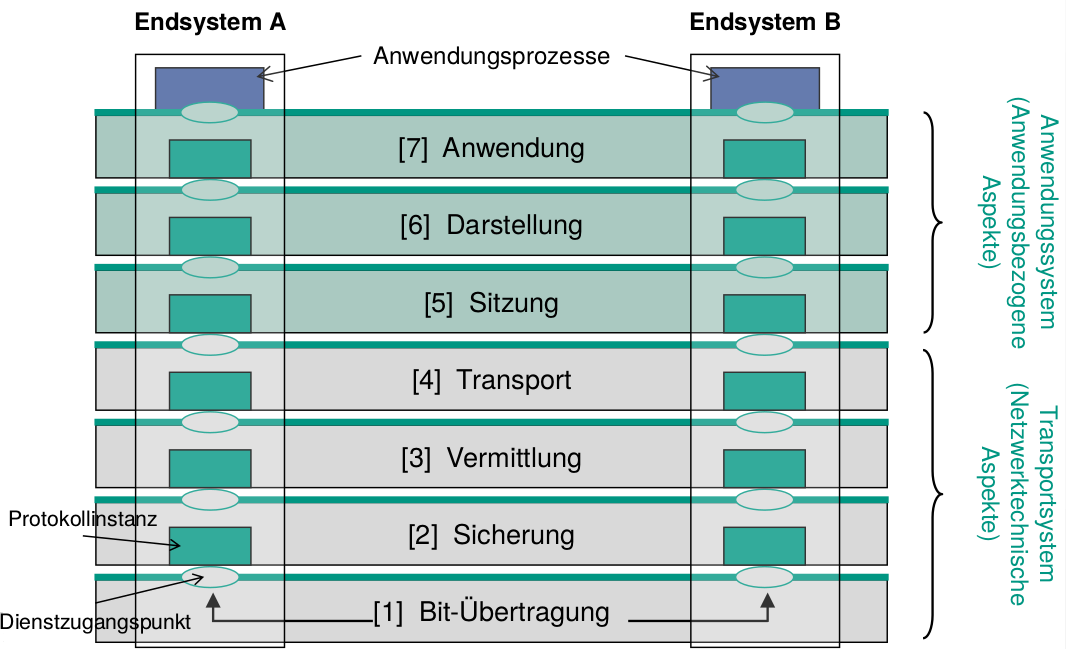
\includegraphics[width=0.4\textwidth]{OSI}\end{figure}
%\begin{figure}[H]\centering\label{OSIKapselung}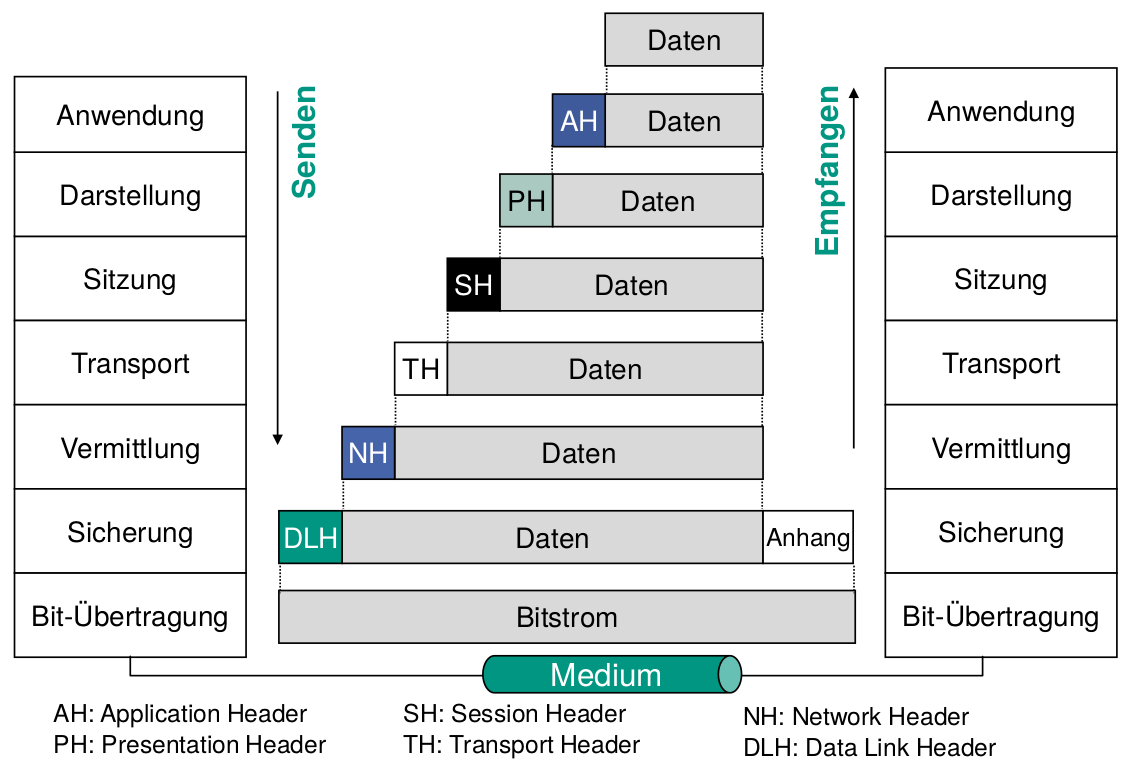
\includegraphics[width=0.33\textwidth]{OSIKapselung}\end{figure}

\newpage

\paragraph{Internet-Referenzmodell}
\begin{items}
  \item Einfachereres Modell, nur 4 Schichten (manchmal 5 bei Trennung von Sicherung und Bit-Übertragung)
  \item Darstellungs- und Sitzungsaufgaben in Anwendungen verlagert
\end{items}
\begin{figure}[H]\centering\label{Internetmodell}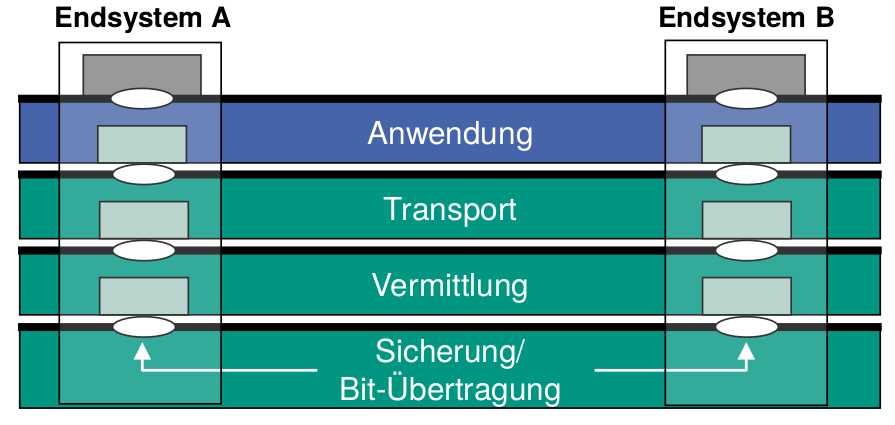
\includegraphics[width=0.33\textwidth]{Internetmodell}\end{figure}

\paragraph{Datenkapselung}
\begin{items}
	\item Information wird durch alle Schichten durchgereicht
	\item Daten werden in jeder Schicht gekapselt (mit Header und/oder Trailer versehen)
\end{items}
\begin{figure}[H]\centering\label{KapselungInternet}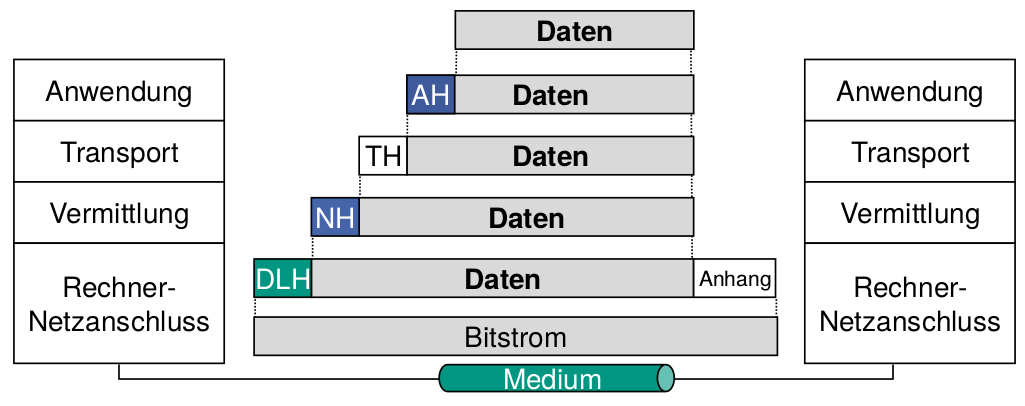
\includegraphics[width=0.33\textwidth]{KapselungInternet}\end{figure}

\paragraph{Protokolle und Dienste}
\begin{items}
  \item \textbf{Protokoll}: Regeln und Formate für Datenaustausch \emph{innerhalb} einer Schicht
  \item \textbf{Dienst}: Bündelung zusammengehöriger Funktionen \\*
    - Zusammenwirkung von Protokollinstanzen \emph{innerhalb} einer Schicht \\*
    - Schichten gehen über gesamtes Kommunikationssystem hinweg\\*
    - \emph{Dienstfunktion}: einzelne Dienstteile unabhängig voneinander nutzbar \\*
    - \emph{Dienstprimitiv}: Einzelvorgänge einer Dienstfunktion \\*
      \phantom{-} \( \cdot \) \emph{request} (Req) --- Beauftragung (Nehmer \( \to \) Geber) \\*
      \phantom{-} \( \cdot \) \emph{indication} (Ind) --- Partnerbenachrichtigung (Nehmer \( \leftarrow \) Geber) \\*
      \phantom{-} \( \cdot \) \emph{response} (Rsp) --- Partnerbeantwortung (Nehmer \( \to \) Geber) \\*
      \phantom{-} \( \cdot \) \emph{confirmation} (Cnf) --- Abschlussbenachrichtigung (Nehmer \( \leftarrow  \) Geber) \\*
    - \emph{Dienstehierarchie}: Dienst baut auf anderen Diensten auf (Dienstbringer/-nehmer) \\*
    - \emph{Dienstzugangspunkte}: Dienstschnittstellen
\end{items}

\paragraph{Ablauf --- Webseitenaufruf}
\begin{items}
  \item \textbf{Start}: Einstecken Netzwerkkabel
  \item \textbf{Ende}: Seitenempfang
  \item \textbf{Netzverbindung}: IP erhalten, Router + DNS kennenlernen \\*
    1. DHCP-Anfrage (verpackt in UDP, IP, 802.3) \\*
    2. Ethernet-Paket wird im LAN gebroadcastet \\*
    3. DHCP-Server im Router empfängt + entpackt Paket \\*
    4. DHCP-Server erstellt DHCP ACK-Paket mit Client-IP, Router-IP, DNS-IP \\*
    5. DHCP-Antwort wird verpackt und direkt an Client gesendet \\*
    6. Client empfängt und entpackt Paket
  \item \textbf{ARP}: MAC des Routers kennenlernen \\*
    1. ARP-Anfrage an Broadcast-Adresse \\*
    2. Router sendet seine MAC in ARP-Antwort
  \item \textbf{DNS}: IP-Adresse der angeforderten Webseite kennenlernen \\*
    1. IP-Datagramm mit DNS-Anfrage wird von LAN-Switch zu lokalem Router geleitet \\*
    2. IP-Datagramm: lokales Netz \( \to \) ISP-Netz \( \to \) DNS-Server (mit RIP oder OSPF) \\*
    3. Paket wird an DNS-Server entpackt \\*
    4. DNS-Server antwortet Client mit angeforderter IP
  \item \textbf{TCP}: Aufbau einer TCP-Verbindung \\*
    1. Eröffnung eines TCP-Sockets zum Webserver \\*
    2. TCP-SYN-Segment wird zu Server geroutet \\*
    3. Server antwortet mit SYNACK
  \item \textbf{HTTP}: Webseite laden \\*
    1. HTTP-Anfrage wird per TCP-Socket gesendet \\*
    2. IP-Datagramm mit HTTP-Anfrage wird zu Webserver geroutet \\*
    3. Server antwortet mit HTTP-Antwort \\*
    4. IP-Datagramm mit HTTP-Antwortet wird zurück zu Client geroutet
\end{items}